\chapter{SU(5), Multiplets, and Proton Decay}

These notes follow Leonard Susskind's lecture on grand unification, with curation by LazyingArt LLC, and they keep the lecture's order of discovery rather than replacing it with a finished textbook taxonomy. The subject is not grand unified theories in full generality, but one concrete example: \(SU(5)\). The lecture begins by insisting that we cannot even state the particle content cleanly until the representation theory is in place. Only after that warmup do we turn to the Standard Model family, the new gauge bosons, proton decay, and finally the numerical relation to supersymmetry through the running of coupling constants.

\section{SU(5) as a Concrete Grand-Unification Example}

The lecture begins by narrowing the target. We are not going to classify all possible grand unified theories. We are going to take one of them apart and see what makes it attractive, what makes it dangerous, and why supersymmetry enters only as a later numerical companion.

The basic group-theoretic claim is that the Standard Model gauge group sits naturally inside a larger simple group,
\begin{equation}
SU(3)\times SU(2)\times U(1)\subset SU(5).
\end{equation}
In that sense grand unification is first of all an exercise in group theory: one looks for a single larger symmetry that contains the separate color and electroweak symmetries as substructures.

At the same time the lecture is careful not to oversell the relation to supersymmetry. The point is not that supersymmetry implies grand unification, nor that grand unification implies supersymmetry. The point is milder and more empirical: if one puts the two ideas together, certain numerical fits improve.

So the first real task is to understand what kinds of representations \(SU(N)\) has, how they combine, and how reducible products split into smaller pieces that transform among themselves.

\section{The Defining Representation, Its Conjugate, and Tensor Products}

For \(SU(N)\) the defining representation is the space of \(N\)-component complex columns,
\begin{equation}
\psi=
\begin{pmatrix}
\psi_1\\
\psi_2\\
\vdots\\
\psi_N
\end{pmatrix},
\end{equation}
acted on by \(N\times N\) special unitary matrices. In components we may write
\begin{equation}
\psi'_i = U_{ij}\psi_j.
\end{equation}
This is the basic \(N\)-dimensional representation, often simply called \(N\).

The first new representation we can make from it is the complex conjugate one. If we take
\[
\psi_i^*,
\]
then these components transform not with \(U\) but with \(U^*\):
\begin{equation}
\psi_i^{*\prime} = U_{ij}^*\psi_j^*.
\end{equation}
This is the conjugate representation, usually denoted \(\bar N\). The lecture emphasizes that, at this level, it is partly a matter of convention which column we think of as the particle representation and which one as the antiparticle representation; once the convention is chosen, however, we must stick to it.

The next thing to do is to combine representations. If one particle transforms as \(N\) and another also transforms as \(N\), then the two-particle system carries a tensor-product representation. Writing the two factors as \(\psi_i\) and \(\phi_j\), we can organize the combined object as
\begin{equation}
\Psi_{ij}=\psi_i\phi_j,
\end{equation}
so that \(\Psi_{ij}\) lives in \(N\otimes N\). Its transformation law is obtained by rotating each index separately:
\begin{equation}
\Psi'_{ij}=U_{ik}U_{j\ell}\Psi_{k\ell}.
\end{equation}

This product has \(N^2\) components, but the lecture immediately warns us that this does not mean it is irreducible. A reducible representation is one that contains smaller sets of linear combinations that transform among themselves and do not mix with the rest. The simplest place where that becomes vivid is the decomposition into symmetric and antisymmetric two-index tensors.

\section{Symmetric and Antisymmetric Two-Index States}

The lecture takes the familiar \(SU(2)\) spin story as the cleanest example of what is going on. Before that example is stated abstractly, the board records the key condition for the symmetric sector.

\begin{figure}
\centering

\includegraphics[width=0.72\textwidth]{lecture_10_figure_02.png}
\caption{Symmetric two-index state condition on the board.}
\end{figure}

The symmetric subspace is defined by
\begin{equation}
\Psi_{ij}=\Psi_{ji},
\end{equation}
and the antisymmetric subspace by
\begin{equation}
\Psi_{ij}=-\Psi_{ji}.
\end{equation}
What matters is that these two sectors do not mix under the group action. Indeed, if \(\Psi_{ij}=\pm \Psi_{ji}\), then
\begin{align}
\Psi'_{ji}
&=U_{jk}U_{i\ell}\Psi_{k\ell} \\
&=U_{ik}U_{j\ell}\Psi_{\ell k} \\
&=\pm U_{ik}U_{j\ell}\Psi_{k\ell} \\
&=\pm \Psi'_{ij}.
\end{align}
Thus the symmetric and antisymmetric subspaces are each invariant under the group. That is exactly what one means here by irreducible pieces sitting inside a reducible tensor product.

For \(SU(2)\), the standard spin-\(\tfrac12\) example becomes
\begin{equation}
2\otimes 2 = 3\oplus 1.
\end{equation}
The four raw states are
\[
|uu\rangle,\qquad |ud\rangle,\qquad |du\rangle,\qquad |dd\rangle.
\]
These reorganize as a symmetric triplet,
\begin{align}
|1,1\rangle &= |uu\rangle,\\
|1,0\rangle &= \frac{1}{\sqrt2}\bigl(|ud\rangle+|du\rangle\bigr),\\
|1,-1\rangle &= |dd\rangle,
\end{align}
and an antisymmetric singlet,
\begin{equation}
|0,0\rangle=\frac{1}{\sqrt2}\bigl(|ud\rangle-|du\rangle\bigr).
\end{equation}
This is the lecture's first real bridge from abstract representation theory to physics. Two spin-\(\tfrac12\) objects do indeed give four raw states, but those four states are not the final story. The group reorganizes them into one three-dimensional multiplet and one one-dimensional multiplet.

\subsection{Question \& Answer}

Why do two \(N\)-plets give \(N^2\) states without violating the exclusion principle?

Because the lecture is not putting two fermions into the same complete quantum state. It is explicitly imagining two distinguishable slots: one particle is here, the other is there. Their positions are different, and the internal \(SU(N)\) labels are being discussed in isolation from position, momentum, and the rest of the quantum numbers. The Pauli principle forbids two identical fermions from occupying the same full state. It does not forbid two spatially separated objects from carrying the same internal label. With that understood, the tensor product really does have \(N^2\) independent components.

\section{From \texorpdfstring{$N\otimes \bar N$}{N x Nbar} to the Adjoint, and Then to the Five-Plet}

The next product is not particle with particle, but particle with antiparticle. The board makes the conceptual move very starkly: \(N\times \bar N\) is to be thought of as a matrix.

\begin{figure}
\centering

\includegraphics[width=0.62\textwidth]{lecture_10_figure_04.png}
\caption{The mixed product \(N\times\bar N\) written as a matrix object on the board.}
\end{figure}

The precise board letter under the product is not perfectly secure, so we write the object cleanly as
\begin{equation}
M_{ij}\in N\otimes \bar N.
\end{equation}
The important point is not the letter but the matrix viewpoint. Once \(M\) is regarded as an \(N\times N\) matrix, there is a natural split into trace and traceless parts:
\begin{equation}
M_{ij}
=
\frac{1}{N}(\operatorname{tr}M)\,\delta_{ij}
+
\left(
M_{ij}-\frac{1}{N}(\operatorname{tr}M)\,\delta_{ij}
\right).
\end{equation}
The first term is a singlet. The second is traceless, and it transforms as the adjoint representation. Thus
\begin{equation}
N\otimes \bar N = 1\oplus \mathrm{Adj},
\qquad
\dim \mathrm{Adj}=N^2-1.
\end{equation}
For \(SU(3)\), this is the familiar statement that quark-antiquark quantum numbers split into a singlet plus an octet, and the octet is precisely where the gluons live.

Only after this toolkit is in hand does the lecture turn to \(SU(5)\) itself. A single Standard Model family is now to be organized into \(SU(5)\) multiplets. The first five-component column is
\begin{equation}
\overline{\mathbf 5}
=
\begin{pmatrix}
\nu\\
e^-\\
\bar d_r\\
\bar d_g\\
\bar d_b
\end{pmatrix},
\end{equation}
where, from now on, the fields are understood as left-handed unless stated otherwise.

\paragraph{A note on convention.}
In standard \(SU(5)\) notation the left-handed family is usually written as \(\overline{\mathbf 5}\oplus \mathbf{10}\). The lecture's spoken and blackboard conventions occasionally sound like the conjugate choice \(\mathbf 5\oplus \overline{\mathbf{10}}\). Rather than drift back and forth, we keep the physical left-handed family in the convention \(\overline{\mathbf 5}\oplus \mathbf{10}\), and we translate the board language as needed.

The lecture also pauses to explain why all particles are being listed as left-handed. The reason is bookkeeping. The antiparticle of a right-handed field is left-handed, so by listing left-handed particles and left-handed antiparticles we do not lose anything. This is especially important because the group representations under discussion are chiral: they do not simply mix left- and right-handed fields into one another.

\subsection{Question \& Answer}

Why does this five-plet contain \(d\)-anti-quarks rather than \(d\)-quarks?

The lecture's answer is a group-theoretic one. Electric charge must be represented by a generator inside the group, and the generators of \(SU(N)\) are traceless Hermitian matrices. One clean way to display that is to write a group element as
\begin{equation}
U=e^{i\theta^a T^a}.
\end{equation}
Because \(U\in SU(N)\), it has determinant one:
\begin{equation}
1=\det U = \exp\!\bigl(i\theta^a \operatorname{tr}T^a\bigr).
\end{equation}
So the generators may be taken traceless:
\begin{equation}
(T^a)^\dagger=T^a,\qquad \operatorname{tr}T^a=0.
\end{equation}
If electric charge is one such generator, then the charge eigenvalues across a multiplet must add to zero.

A clean reconstruction of the lecture's charge argument is therefore
\begin{equation}
Q=\mathrm{diag}\!\left(0,-1,\frac13,\frac13,\frac13\right),
\qquad
\operatorname{tr}Q=0.
\end{equation}
Indeed,
\begin{equation}
0+(-1)+3\left(\frac13\right)=0.
\end{equation}
If we had tried to put \(d\)-quarks in the multiplet instead of \(\bar d\)-quarks, the sum would have been
\[
0+(-1)+3\left(-\frac13\right)=-2,
\]
and charge could not be embedded into the traceless generators of \(SU(5)\) in the way the lecture wants. This is the mathematical reason the strange-looking choice is not optional.

\section{The Antisymmetric Matrix and the Remaining Fermions}

At this point the five-component multiplet is visibly incomplete. Where are the up quarks? Where is the positron? Where are the remaining left-handed fields of the family? The lecture answers this not by announcing the final result from above, but by performing what Susskind himself calls a bit of group-theory gymnastics.

The board next turns to the conjugate five-component column with quantum numbers
\begin{equation}
\chi=
\begin{pmatrix}
\bar\nu\\
e^+\\
d_r\\
d_g\\
d_b
\end{pmatrix}.
\end{equation}
Because the lecture's conjugation language drifts, it is better here to trust the quantum numbers rather than the overbar on the representation label. The move itself is clear: take the antisymmetric part of the tensor square of this five-component object.

\begin{equation}
\Psi_{ij}=-\Psi_{ji},
\qquad
\Psi_{ii}=0.
\end{equation}
The diagonal entries vanish, and the lower triangle is fixed by the upper triangle. Therefore the number of independent entries is
\begin{equation}
\frac{5\cdot 4}{2}=10.
\end{equation}
That is the ten-dimensional multiplet we were looking for.

The board snapshot is important here because it shows not only the antisymmetric matrix itself but also the visible \(2\oplus 3\) split between the lepton-like slots and the color slots.

\begin{figure}
\centering

\includegraphics[width=0.86\textwidth]{lecture_10_figure_05.png}
\caption{The antisymmetric \(5\times 5\) matter matrix on the board, with the visible \(2\oplus 3\) block split.}
\end{figure}

A clean reconstruction, faithful to the lecture's content though not to every obscured sign on the board, is
\begin{equation}
\Psi \sim
\left(
\begin{array}{cc|ccc}
0 & e^+ & d_r & d_g & d_b\\
-e^+ & 0 & u_r & u_g & u_b\\
\hline
-d_r & -u_r & 0 & \bar u_b & \bar u_g\\
-d_g & -u_g & -\bar u_b & 0 & \bar u_r\\
-d_b & -u_b & -\bar u_g & -\bar u_r & 0
\end{array}
\right),
\qquad
\Psi_{ij}=-\Psi_{ji}.
\end{equation}
The precise sign convention in the lower \(3\times 3\) block is partly a matter of antisymmetry and partly hidden by the board occlusion, so one should not overclaim there. What is stable is the structure: the \((1,2)\) slot carries the quantum numbers of \(e^+\); the first row and first column beyond the first two slots carry the three \(d\)-quarks; the second row and column beyond the first two slots carry the three \(u\)-quarks; and the lower \(3\times3\) antisymmetric color block carries the quantum numbers of the three \(\bar u\)-quarks.

This lower color block is also where the lecture uses the old color-combination trick. An antisymmetric pair of colors behaves like an anti-color. Thus the antisymmetric color pairs naturally produce \(\bar u_r\), \(\bar u_g\), and \(\bar u_b\). In this way the entire first family fits into
\begin{equation}
\overline{\mathbf 5}\oplus \mathbf{10}.
\end{equation}
That is the remarkable structural fact the lecture wants us to stare at for a moment before moving on. The fit is mathematically neat, but it is also rather odd: some particles and their antiparticles sit in the same grand-unified structure, while others live in different representations. The uneasiness is part of the point.

\section{Gauge Bosons as Shifts and the Appearance of Proton Decay}

After the matter multiplets have been organized, the lecture changes gear. It is no longer enough to know where the particles sit. We now want to know what the gauge bosons do.

In the five-component column the gauge bosons are simply the agents of the allowed transitions among the five slots. The familiar ones already occupy obvious places: the electroweak bosons act in the upper \(2\times 2\) sector, and the gluons act in the lower \(3\times 3\) color sector. The new ingredients are the bosons that move between these blocks. Those are the leptoquark gauge bosons customarily called \(X\) and \(Y\).

A compact schematic version of the lecture's shift picture is the following.

\begin{figure}
\centering
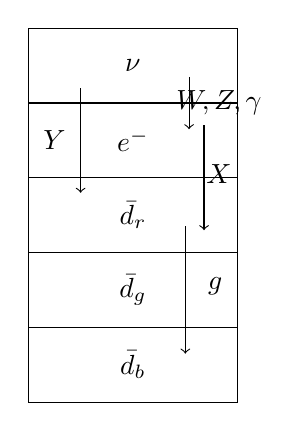
\begin{tikzpicture}[scale=0.95]
\draw (0,0) rectangle (2.8,5);
\draw (0,4) -- (2.8,4);
\draw (0,3) -- (2.8,3);
\draw (0,2) -- (2.8,2);
\draw (0,1) -- (2.8,1);

\node at (1.4,4.5) {$\nu$};
\node at (1.4,3.5) {$e^-$};
\node at (1.4,2.5) {$\bar d_r$};
\node at (1.4,1.5) {$\bar d_g$};
\node at (1.4,0.5) {$\bar d_b$};

\draw[->] (2.15,4.35) -- (2.15,3.65);
\node at (2.55,4.0) {$W,Z,\gamma$};

\draw[->] (2.1,2.35) -- (2.1,0.65);
\node at (2.5,1.55) {$g$};

\draw[->] (0.7,4.2) -- (0.7,2.8);
\node at (0.35,3.5) {$Y$};

\draw[->] (2.35,3.7) -- (2.35,2.3);
\node at (2.55,3.05) {$X$};
\end{tikzpicture}
\caption{Gauge bosons as shifts among the five slots: electroweak in the upper block, color in the lower block, and \(X,Y\) between the two.}
\end{figure}

The lecture is explicit about the charges but cautious about the names. The bosons that connect leptons to color-carrying states come with charges \(\pm \tfrac43\) and \(\pm \tfrac13\), but Susskind says outright that he does not remember which label, \(X\) or \(Y\), belongs to which charge assignment. What should be preserved is the transition pattern, not a spurious certainty about the names.

The same generators then act on the ten-dimensional antisymmetric multiplet. Here the lecture's picture is that a gauge boson acts as a shift on one index or the other. Therefore, in the matrix, the action appears as a horizontal or vertical move. A gluon can move us among colors along a row or along a column. A weak boson can move us between the first two slots, and in doing so it induces the familiar \(d\to u\) weak transition inside the larger antisymmetric matrix. The leptoquark bosons do the same sort of thing, but now between the upper two and lower three sectors.

Once those shifts exist, genuinely new processes exist. In particular, one can convert a quark into a lepton and another quark into an antiquark. That is the conceptual seed of proton decay.

At the level of channels, the lecture's main example is
\begin{equation}
p\to e^+ + \pi^0,
\end{equation}
with the secondary possibility
\begin{equation}
p\to e^+ + \gamma.
\end{equation}
The logic is simple. Start with a proton, \(uud\). Use an \(X\)- or \(Y\)-type boson to convert one quark into a positron and another into an antiquark; the remaining quark acts as a spectator. The quark-antiquark pair can hadronize into a neutral pion, or less likely annihilate into a photon.

This is the dramatic turn of the lecture. The same symmetry that made the multiplets look beautiful also makes ordinary matter unstable unless something suppresses the new processes very strongly.

\subsection{Question \& Answer}

If the new bosons have ordinary-sized couplings, why does the proton not decay immediately?

The lecture's answer is that only the mass scale of the heavy leptoquark bosons can save us. The couplings are not assumed to be fantastically tiny; they are of the same broad order as the ordinary gauge couplings of the unified theory. So the suppression must come from the propagator of the heavy intermediate boson.

At the level of amplitudes, the exchange gives
\begin{equation}
\mathcal A(p\to e^+\pi^0)\sim \frac{g^2}{M_X^2},
\end{equation}
up to numerical coefficients and kinematic factors. Squaring the amplitude to obtain the decay rate gives
\begin{equation}
\Gamma_p \sim \frac{g^4}{M_X^4}
\end{equation}
again up to additional factors involving the proton mass and hadronic matrix elements. The lifetime is the inverse rate,
\begin{equation}
\tau_p\sim \Gamma_p^{-1}.
\end{equation}

The lecture then compares this with experiment. The observational bound is roughly
\begin{equation}
\tau_p \gtrsim 10^{33}\ \text{years}.
\end{equation}
That is absurdly longer than the naive microscopic time scale of a proton, which the lecture estimates by the light-crossing time of a proton, roughly \(10^{-23}\) seconds. So the gap is enormous. The only available lever is the heavy mass in the propagator. Order-of-magnitude reasoning therefore pushes the new boson masses to
\begin{equation}
M_X \sim 10^{15}\text{--}10^{16}\,\mathrm{GeV},
\end{equation}
and the lecture settles on the memorable scale
\begin{equation}
M_X \gtrsim 10^{16}\,\mathrm{GeV}.
\end{equation}
That is the sense in which proton decay is both a prediction and a threat. The theory wants the process, but only at a rate so tiny that matter survives.

\section{Unification Scale, Running Couplings, and the Supersymmetry Epilogue}

The lecture is not content to leave the scale \(10^{16}\,\mathrm{GeV}\) as a number extracted only from proton stability. It asks whether the same scale appears elsewhere.

The next point is that \(SU(5)\) cannot be an unbroken symmetry of nature. If it were unbroken, the \(X\) and \(Y\) bosons would sit in the same multiplet as the gluons, the \(W\), the \(Z\), and the photon, and they would not be allowed to have this gigantic mass while the others remain light or massless. So a separate high-scale Higgs mechanism is required to split the upper \(2\)-block from the lower \(3\)-block and to give the leptoquark bosons their enormous masses. Above that symmetry-breaking scale, however, one expects the full \(SU(5)\) symmetry to be restored as a good approximation.

That leads directly to the running of coupling constants. Instead of treating the strong, weak, and electromagnetic couplings as fixed numbers, we let them run with energy. The lecture phrases this graphically, in terms of plotting the inverse couplings against the logarithm of the energy:
\begin{equation}
\alpha_1^{-1}(\mu),\qquad \alpha_2^{-1}(\mu),\qquad \alpha_3^{-1}(\mu).
\end{equation}
The three curves do not meet perfectly in the minimal nonsupersymmetric picture, but they come tantalizingly close. The near-crossing occurs at an energy scale of order
\begin{equation}
\mu \sim 10^{15}\text{--}10^{16}\,\mathrm{GeV},
\end{equation}
which is precisely the scale that proton stability was already hinting at.

So the lecture closes the circle. Proton decay wants the new bosons to be extremely heavy. Running couplings suggest that the place where the separate Standard Model couplings begin to look unified is again around \(10^{15}\) to \(10^{16}\,\mathrm{GeV}\). Supersymmetry then enters only as an empirical epilogue: if one includes the superpartner spectrum in the running, the three couplings meet much more cleanly, at the level of about a percent. That does not establish either supersymmetry or grand unification as a theorem. It simply makes the coincidence more compelling.

The lecture also remarks, briefly, that a still larger group can do even better at the level of representation theory. In a bigger unification, usually written \(SO(10)\), a whole family can be placed in a single sixteen-dimensional multiplet, provided one adds the right-handed neutrino. But that is left for another story.

\section{Summary}

The lecture's structure is deliberate. We begin with \(SU(N)\) representation theory because without it the particle story cannot be stated cleanly. The defining representation \(N\), its conjugate \(\bar N\), the symmetric and antisymmetric pieces of \(N\otimes N\), and the singlet plus adjoint decomposition of \(N\otimes \bar N\) are not decorative preliminaries. They are the machinery that lets one see how a Standard Model family can be organized inside \(SU(5)\).

Once that machinery is in place, the family fits into the familiar pattern
\[
\overline{\mathbf 5}\oplus \mathbf{10},
\]
with the five-component multiplet containing \(\nu\), \(e^-\), and the three \(\bar d\)'s, and the ten-dimensional antisymmetric multiplet carrying the remaining fermions. The same group structure also forces new gauge bosons, and these in turn force proton decay unless they are very heavy.

That is why the lecture ends where it does: at the scale \(10^{15}\) to \(10^{16}\,\mathrm{GeV}\), where proton stability, high-scale symmetry breaking, and the near-unification of the running couplings all begin to point in the same direction. Supersymmetry does not generate that logic, but it sharpens the numerical fit. The resulting picture is mathematically beautiful, physically dangerous, and therefore worth taking seriously.